\chapter{Ala i estabilitzadors}

Un cop estudiat el comportament de l'ala aïllada, s'ha d'estudiar el comportament del planejador complet, tenint en compte tant l'estabilitzador horitzontal com el vertical i, per tant, les interaccions i interferències que aixo produeix respecte l'ala aïllada.

Per tal d'estudiar el conjunt, s'assumeix que l'estabilitzador vertical té un angle de torsió $\theta$ nul. A més, s'estableix que l'estabilitzador horitzontal només produeix resistència aerodinàmica paràsita ja que presenta un angle de lliscament $\beta=0^{\circ}$ i per tant no genera sustentació ni conseqüentment resistència induïda.

La geometria del planejador sencer s'il·lustra a la figura \ref{glider}

 \begin{figure}[H]
 	\centering
 	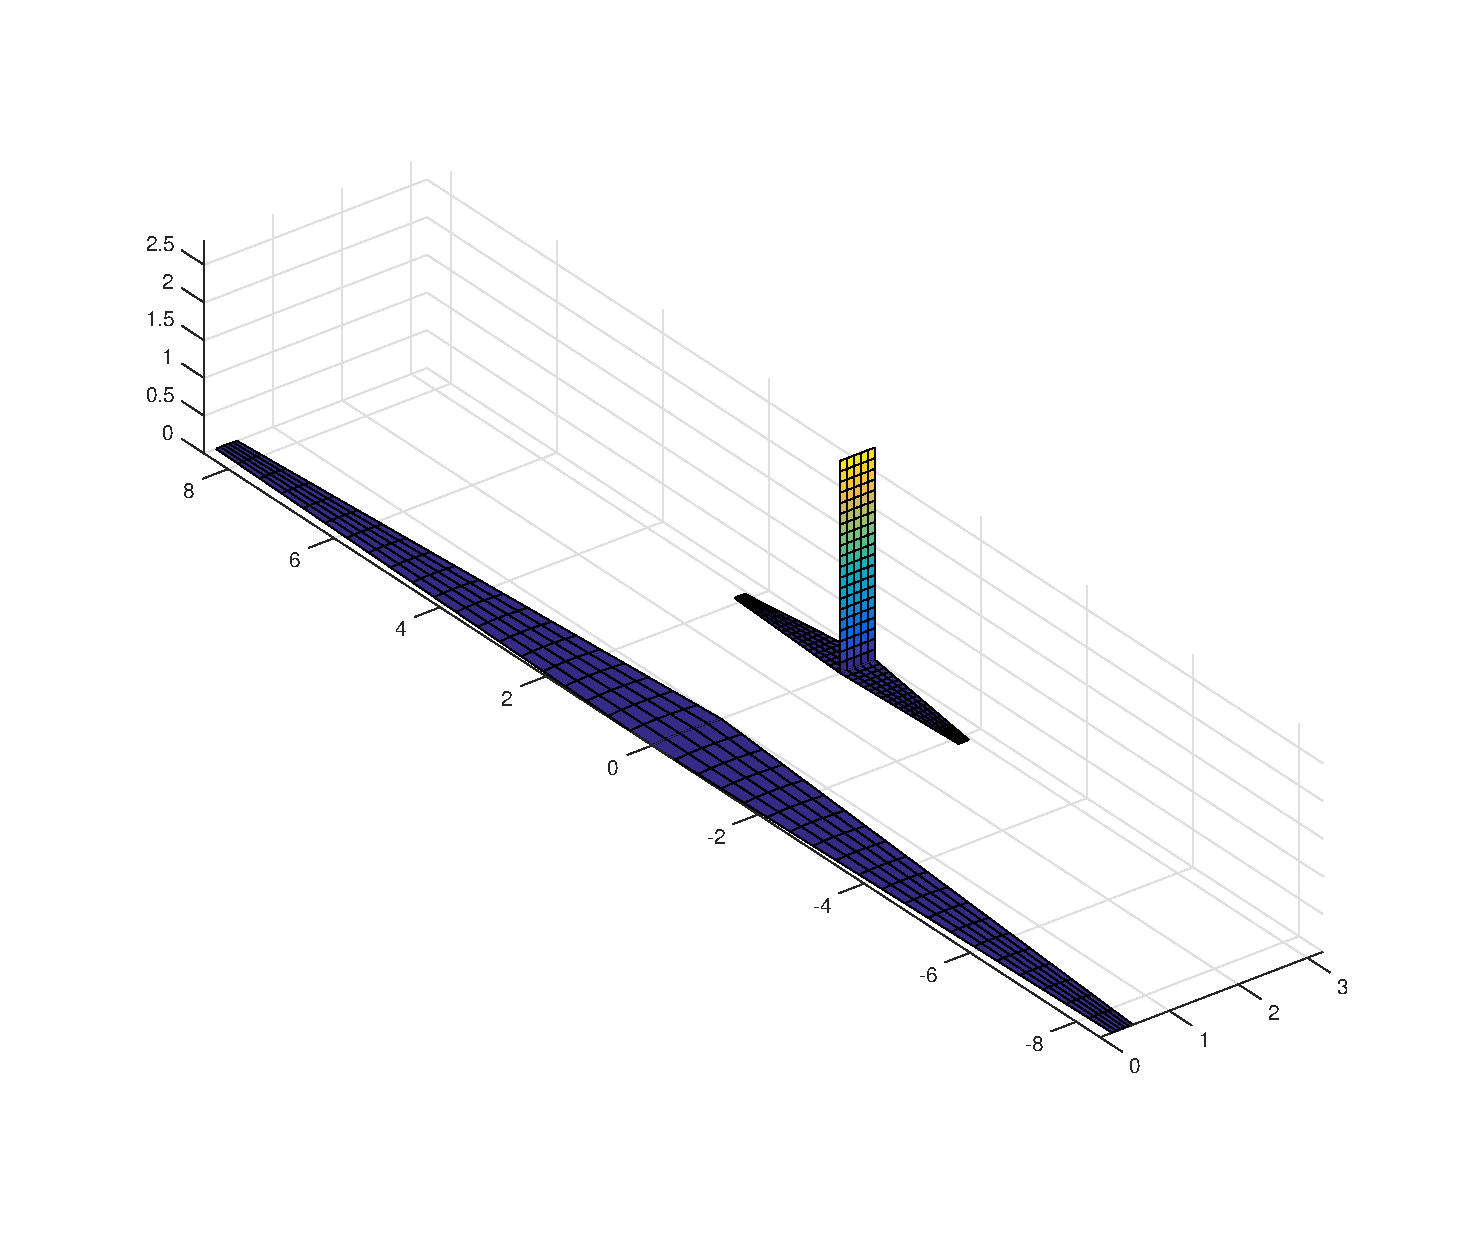
\includegraphics[width=0.8\textwidth]{./plots/glider}
 	\caption{Configuració geomètrica del planejador}
 	\label{glider}
 \end{figure}

\section{Coeficients aerodinàmics}

Amb l'objectiu d'estudiar el comportament del conjunt ala-estabilitzadors, es calcula tant el coeficient de sustentació com el de resistència per una configuració de vol amb un angle d'atac de valor $\alpha=6^{\circ}$. 

Els resultats obtinguts són $\bm{C_{L} = 0.859} $ i $\bm{C_{D} = 0.027} $.


\section{Posició del centre de masses}

Finalment, s'estudia l'estabilitat del planejador. Per fer-ho es calcula la posició del centre de masses que fa que el conjunt ala-estabilitzadors sigui longitudinalment estable. 

Per realitzar el càlcul s'agafa la configuració d'angle d'atac vista a l'apartat anterior, $\alpha=6^{\circ}$, i s'imposa que el sumatori de moments respecte el centre de masses (punt a trobar) sigui igual a zero. L'algoritme seguit per fer-ho es mostra a la figura \ref{AlgoritmeCM}.

\begin{figure}[H]
	\centering
	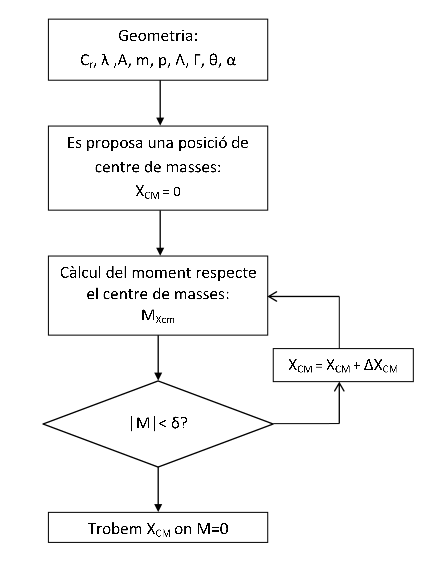
\includegraphics[scale=0.5]{./plots/algoritmeCM}
	\caption{Algoritme de càlcul de la posició del centre de masses}
	\label{AlgoritmeCM}
\end{figure}

Com es pot observar, es tracta d'un algoritme iteratiu. Per tant, un cop definida la geometria, es proposa una distancia de centre de masses per a que el programa pugui a començar a calcular i es calculen els moments respecte aquest punt proposat, comprovant que el resultat sigui més petit que una tolerància. En aquest cas com que el que es busca és el punt respecte el qual els moments són zero, aquesta tolerància es de $\delta=10^{-9}$. Si aquesta condició no es compleix, es varia la distancia del centre de masses en un increment que depèn del valor de moments obtingut. El procés es repeteix fins que s'obté el valor buscat. 

Així doncs, un cop realitzats els càlculs s'obté  que $\bm{X_{CM} = 0.1659}$.

\section{Efecte terra: Planejador}
Si la configuració anterior s'apropa al terra de forma que $h = \overline{c}$ apareix l'efecte terra. Així doncs, per obtenir les noves circulacions, s'aplica el mètode de les imatges similarment a com es proposa a la secció \ref{gndAlg}. A partir d'aquí, es torna a computar la sustentació, la resistència  i el moment respecte del centre de masses trobat a l'anterior apartat.
\begin{figure}[H]
	\centering
	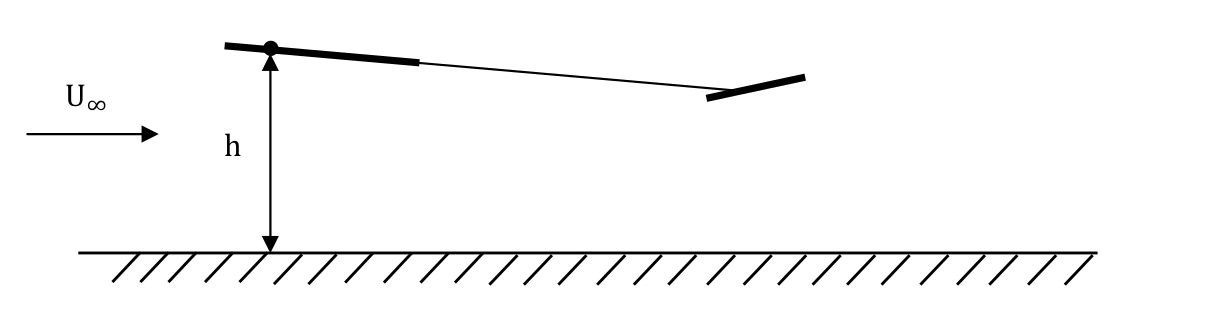
\includegraphics[scale=0.35]{./plots/terraGlider}
	\caption[Esquema de la posició de l'ala sobre el terra ($h=\bar{c}$)]{Esquema de la disposició del planejador a prop del terra ($h=\bar{c}$) \cite{LizandraDalmases2017a}}
	\label{GroundEffectGlider}
\end{figure}

Fixant un angle d'atac de 6$^{\circ}$, es comparen els resultats dels coeficients aerodinàmics de l'avió complet pel cas sense efecte terra i pel cas amb efecte terra.
\begin{table} [H]
	\centering
	\begin{tabular}{| c | c | c |}	
		\hline
		& $C_{L}$ & $C_{D}$  \\
		\hline
		Sense efecte terra & 0.8595 & 0.0271 \\
		\hline
		Amb efecte terra & 0.9541 & 0.0177 \\
		\hline
		Variació & 11\% & -34.57\% \\
		\hline
	\end{tabular}
\caption{Variació dels coeficients amb i sense efecte terra} \label{NoGroundvsGroundGlider}
\end{table}
Novament, els resultats obtinguts són físicament coherents, doncs l'efecte terra fa incrementar lleugerament la sustentació.

Per últim, el moment respecte del centre de masses trobat a l'apartat anterior s'ha computat obtenint $\bm{C_{M_{cm}} = -0.0992 }$.
